%%%%%%%%%%%%%%%%%%%%%%%%
%
% $Autor: Sudhanshu Pukale $
% $Datum: 2025-03-08 $
% $Pfad: GitHub/ML24-EX02-Pico4ML/Pico4ML-BLE/Contents/General/ICM20948.tex $
% $Version: 1 $
%
%%%%%%%%%%%%%%%%%%%%%%%%



\chapter{IMU ICM-20948}

\section{Introduction}

Microelectromechanical electro mechanical systems \index{(MEMS)} inertial devices have many advantages such as low cost, small size, light weight, low power consumption,and easy large-scale production, and have been widely used in the field of inertial navigation. However, the measurement accuracy and reliability are low, which cannot be ignored. Therefore, it is an important research direction to improve the accuracy of MEMS inertial devices while making full use of their advantages.The use of low cost, low precision and low reliability MEMS inertial devices to manufacture high-precision and high-reliability products, and then achieve high-precision and high-reliability navigation goals, has become a hot topic in the field of inertial navigation.There are two main ways to achieve the above goals, one is to improve the accuracy of a single MEMS inertial device, and the other is to use multiple low-precision MEMS inertial devices to improve the accuracy. As early as 2003, David S. Bayard and Scott R. Ploenin the United States proposed a method for fusing multiple gyroscopes to significantly improve performance.\cite{Treichler:2005} Under the influence of this idea, later researchers in the field of inertial navigation further proposed MEMS virtual gyroscope array [5], accelerometer array, inertial sensor array \cite{Zhu:2014}, IMU arrays, etc., all of which are based on Newton’s law of inertia.\cite{Xuan:2024}

\section{General}

The ICM-20948 is the world’s lowest power 9-axis MotionTracking device that is ideally suited for Smartphones, Tablets, Wearable Sensors, and IoT applications.\cite{TDK:2024}

\begin{itemize}
	\item  3-axis gyroscope, 3-axis accelerometer, 3-axis
	compass, and a Digital Motion Processor™ \index{(DMPTM)}
	in a 3 mm x 3 mm x 1 mm (24-pin QFN) package
	\item DMP offloads computation of motion processing
	algorithms from the host processor, improving
	system power performance
	\item Software drivers are fully compliant with Google’s
	latest Android release
	\item EIS FSYNC support
\end{itemize}

ICM-20948 supports an auxiliary I2C interface to external sensors, on-chip 16-bit ADCs, programmable digital filters, an embedded temperature sensor, and programmable interrupts. The device features an operating voltage range down to 1.71V. Communication ports include I 2C and high speed SPI at 7 MHz.


\section{Specific Sensor/Actor}


\index{IMUs} Inertial Measurement Units measure acceleration, angular velocity and magnetic fields. When these measurements are combined, they help us determine the motion and orientation of an object.\cite{221e:2025}.IMUs consist of three main inertial sensing components: an accelerometer, a gyroscope, and a magnetometer. When combined, these three components offer data that provide a comprehensive view of the system on which they are installed.\ref{ICM-20948}

\textbf{Accelerometers:-}A MEMS accelerometer uses a microstructure suspended by springs to allow movement in response to acceleration.As the accelerometer experiences acceleration, the mass within resists motion due to its inertia, creating an electrical output like voltage or current.By combining readings from its three axes (x, y, and z), corresponding to left-right, up-down, and forward-backward directions, respectively, the accelerometer can accurately determine an object’s motion and orientation in three-dimensional space. This also enables it to characterize and monitor shocks and vibrations.\cite{221e:2025}.\ref{fig:accelerometer_specifications}

\textbf{Gyroscopes:-}When things rotate around an axis, they have what is called angular velocity, this is what a gyroscope measures.A MEMS gyroscope uses a vibrating structure to determine the rate of rotation (i.e., angular velocity), based on the measure of the Coriolis force exerted during the rotation. The Coriolis force is an inertial one exerted on objects in motion/rotation, it makes an object appear to deviate from its path, but in reality it does not.If you tilt a gyroscope forward, it senses an apparent force pushing it in a direction perpendicular to both the rotation axis and the direction of the force you applied. The forward tilt will causes it to move sideways to maintain its original orientation.\cite{221e:2025}.\ref{fig:Gyroscope_specifications}

\textbf{Magnetometers:-}
A magnetometer relies on the Earth’s magnetic field to determine the host object’s orientation relative to the Earth’s magnetic North. When the IMU is properly calibrated, the magnetometer can detect the direction of the Earth’s magnetic field.As the IMU-equipped object moves or rotates, the magnetometer senses this movement. Changes in the magnetic field components along the x, y, and z axes can be related to angular variation with respect to Earth’s magnetic north.An Attitude and Heading Reference System (AHRS) uses magnetometers in conjunction with accelerometers and gyroscopes to provide a more comprehensive and accurate orientation estimation. Gyroscopes measure angular velocity, while accelerometers measure linear acceleration. By combining data from all three sensors, the IMU can track the object’s position, orientation, and movement in three-dimensional space.\cite{221e:2025}..\ref{fig:Magnetometer_specifications}


\begin{figure}[h!]
	\centering
	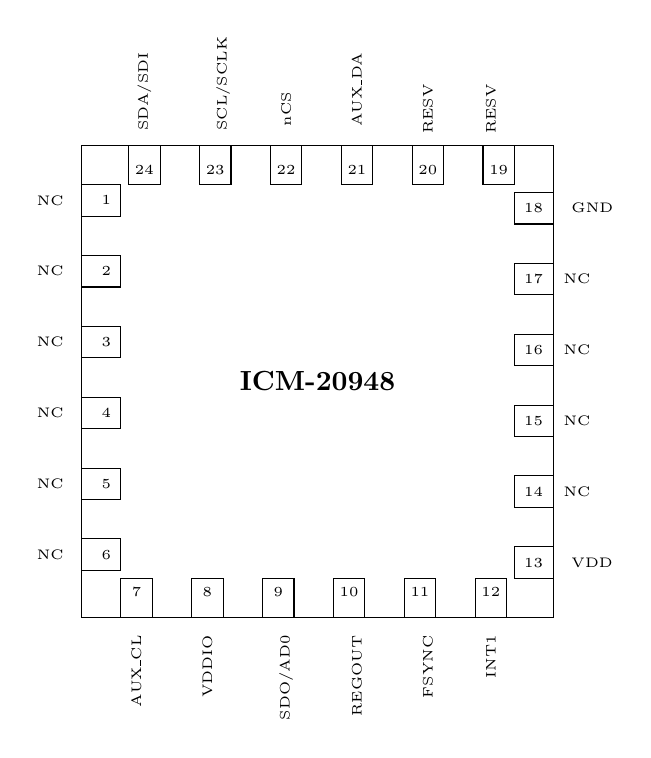
\begin{tikzpicture}[scale=1]
		
		% Main rectangle
		\draw (0,0) rectangle (6,6);
		
		% ICM-20948 Text
		\node at (3,3) {\textbf{ICM-20948}};
		
		% Top pins (REVERSED ORDER)
		\foreach \i [count=\j from 19, evaluate=\j as \x using (\j-19)*0.9] in {19, 20, 21, 22, 23, 24}
		{
			\draw (5.5-\x,6) rectangle (5.1-\x,5.5);
			\node[above] at (5.3-\x,5.5) {\tiny\i};
		}
		
		% Bottom pins
		\foreach \i [evaluate=\i as \x using (\i-7)*0.9] in {7,8,9,10,11,12}
		{
			\draw (0.5+\x,0) rectangle (0.5+\x+0.4,0.5);
			\node[below] at (0.7+\x,0.5) {\tiny\i};
		}
		
		% Left pins
		\foreach \i [evaluate=\i as \y using (\i-1)*0.9] in {1,2,3,4,5,6}
		{
			\draw (0,5.5-\y) rectangle (0.5,5.5-\y-0.4);
			\node[left] at (0.5,5.3-\y) {\tiny\i};
		}
		
		% Right pins
		\foreach \i [evaluate=\i as \y using (\i-13)*0.9] in {13,14,15,16,17,18}
		{
			\draw (6,0.5+\y) rectangle (5.5,0.5+\y+0.4);
			\node[right] at (5.5,0.7+\y) {\tiny\i};
		}
		
		% Pin labels (adjust positions as needed for clarity)
		
		% Top labels
		\node[above,font=\tiny, anchor=east, rotate=90] at (0.8,7.3) {SDA/SDI};
		\node[above,font=\tiny, anchor=east, rotate=90] at (1.8,7.5) {SCL/SCLK};
		\node[above,font=\tiny, anchor=east, rotate=90] at (2.6,6.8) {nCS};
		\node[above,font=\tiny, anchor=east, rotate=90] at (3.5,7.3) {AUX\_DA};
		\node[above,font=\tiny, anchor=east, rotate=90] at (4.4,6.9) {RESV};
		\node[above,font=\tiny, anchor=east, rotate=90] at (5.2,6.9) {RESV};
		
		% Bottom labels
		\node[below,font=\tiny, anchor=east, rotate=90] at (0.7,-0.1) {AUX\_CL};
		\node[below,font=\tiny, anchor=east, rotate=90] at (1.6,-0.1) {VDDIO};
		\node[below,font=\tiny, anchor=east, rotate=90] at (2.6,-0.1) {SDO/AD0};
		\node[below,font=\tiny, anchor=east, rotate=90] at (3.5,-0.1) {REGOUT};
		\node[below,font=\tiny, anchor=east, rotate=90] at (4.4,-0.1) {FSYNC};
		\node[below,font=\tiny, anchor=east, rotate=90] at (5.2,-0.1) {INT1};
		
		% Left labels
		\node[left,font=\tiny] at (-0.1,5.3) {NC};
		\node[left,font=\tiny] at (-0.1,4.4) {NC};
		\node[left,font=\tiny] at (-0.1,3.5) {NC};
		\node[left,font=\tiny] at (-0.1,2.6) {NC};
		\node[left,font=\tiny] at (-0.1,1.7) {NC};
		\node[left,font=\tiny] at (-0.1,0.8) {NC};
		
		% Right labels
		\node[right,font=\tiny] at (6.1,0.7) {VDD};
		\node[right,font=\tiny] at (6.,1.6) {NC};
		\node[right,font=\tiny] at (6.,2.5) {NC};
		\node[right,font=\tiny] at (6.,3.4) {NC};
		\node[right,font=\tiny] at (6.,4.3) {NC};
		\node[right,font=\tiny] at (6.1,5.2) {GND};
		
		
	\end{tikzpicture}
	\caption{ICM-20948 \cite{TDK:2024}}
	\label{ICM-20948}
\end{figure}

\section{Specification}

\textbf{Accelerometer Specifications}

\begin{figure}[h!]
	\centering
	\includegraphics[width=1.2\textwidth]{ICM20948/AcclerometerSpecifications.png}
	\caption{Accelerometer Specifications \cite{TDK:2024}}
	\label{fig:accelerometer_specifications}
\end{figure}

\textbf{Magnetometer Specifications}

\begin{figure}[h!]
	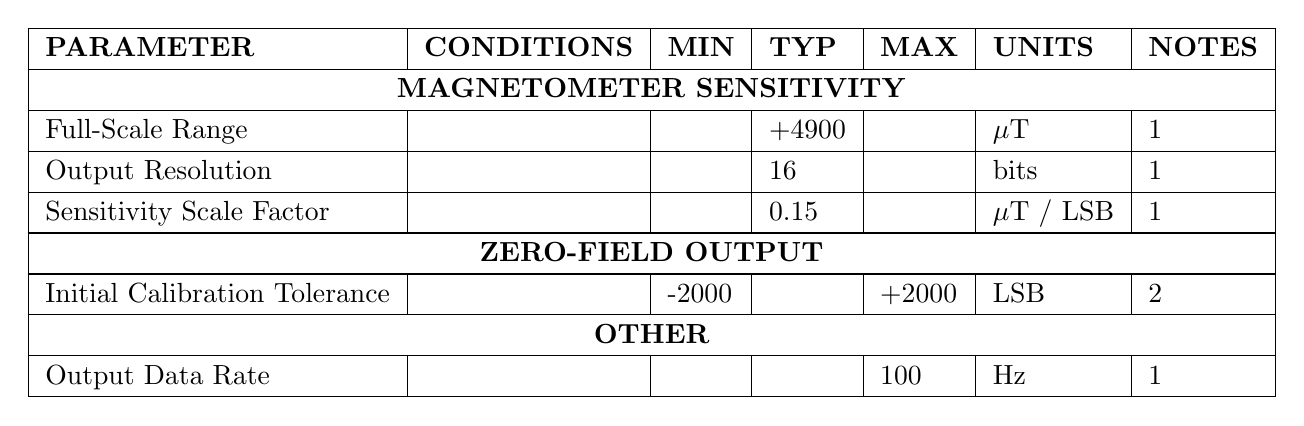
\begin{tikzpicture}
		\node (table) [inner sep=0pt] {
			\begin{tabular}{|l|l|l|l|l|l|l|}
				\hline
				\textbf{PARAMETER} & \textbf{CONDITIONS} & \textbf{MIN} & \textbf{TYP} & \textbf{MAX} & \textbf{UNITS} & \textbf{NOTES} \\
				\hline
				
				\multicolumn{7}{|c|}{\textbf{MAGNETOMETER SENSITIVITY}} \\
				\hline
				Full-Scale Range &  &  & +4900 &  & $\mu$T & 1 \\
				\hline
				Output Resolution &  & & 16 &  & bits & 1 \\
				\hline
				Sensitivity Scale Factor &  & & 0.15 &  & $\mu$T / LSB & 1 \\
				\hline
				\multicolumn{7}{|c|}{\textbf{ZERO-FIELD OUTPUT}} \\
				\hline
				Initial Calibration Tolerance & &-2000 &  &+2000 & LSB & 2 \\
				\hline
				\multicolumn{7}{|c|}{\textbf{OTHER}} \\
				\hline
				Output Data Rate &  &  & & 100 & Hz & 1 \\
				\hline
			\end{tabular}
		};
	\end{tikzpicture}
	\caption{Magnetometer Specifications \cite{TDK:2024}}
	\label{fig:Magnetometer_specifications}
\end{figure}

\textbf{Gyroscope Specifications}

\begin{figure}[h!]
	\centering
	\includegraphics[width=1.2\textwidth]{ICM20948/GyroscopesSpecifications.png}
	\caption{Accelerometer Specifications \cite{TDK:2024}}
	\label{fig:Gyroscope_specifications}
\end{figure}







\newpage
\section{Library}

The term library in programming refers to isolated compiling of already-written codes that may be used by programmers to perform specific tasks or functions without having to write the code from scratch.
These libraries aim at the ease of developers by speeding up the software development process by providing ready-made solutions to some of the most common programming problems. \\

\textbf{Wire.h}\\
Wire.h is a library in Arduino that allows for communication between I2C devices.
I2C stands for Inter-Integrated Circuit, which is a synchronous serial communication
protocol used for connecting microcontrollers to peripheral devices. Wire.h provides
functions for initializing the I2C bus, sending and receiving data over the bus, and
managing multiple devices on the same bus. With this library, developers can easily
connect multiple I2C devices, such as sensors or displays, to an Arduino board.\cite{arduinoWire:2025}

\medskip

\textbf{ICM\_20948\_we.h}
The ICM20948\_WE is an Arduino library for interfacing with the ICM-20948 9-axis sensor, which combines an accelerometer, gyroscope, and magnetometer.It provides a comprehensive set of functions to interact with the ICM-20948 sensor and includes numerous example sketches with detailed comments to facilitate easy implementation.\cite{Ewald:2021}


\section{Calibration}

Calibration of the ICM-20948 IMU involves several steps to ensure accurate readings from its accelerometer, gyroscope, and magnetometer sensors. Here's an overview of the calibration process:

\textbf{Accelerometer Calibration}
\begin{enumerate}
	\item Determine the minimum and maximum raw acceleration values for each axis (X, Y, Z) in the ±2g range.
	
	\item Use these values to set offsets and adjust the slope/ratio of raw acceleration vs. g.\cite{Ewald:2021}
	
	\item The zero point is typically set as (min + max)/2 for each axis
\end{enumerate}

\textbf{Gyroscope Calibration}
\begin{enumerate}
	\item Measure the gyroscope offset values when the sensor is stationary.
	
	\item Apply these offsets to start with zero values when the sensor is not moving.\cite{Ewald:2021}
\end{enumerate}

\textbf{Magnetometer Calibration}

\begin{enumerate}
	\item Rotate the IMU in various orientations to collect data points.
	
	\item Software algorithms then compute calibration parameters based on these measurements
\end{enumerate}
\section{Simple Code}

\begin{code}[h!]
	\captionof{code}{Example IMU Sensor Code}\label{IMU:example}
	\ArduinoExternal{}{../../Code/Pico4ML/IMU/IMU.ino}
\end{code}

\section{Simple Application}
The Pico4ML-BLE, which includes the ICM-20948 IMU sensor, can be used for various applications leveraging its accelerometer, gyroscope, and magnetometer capabilities. Here are some key applications:

\begin{enumerate}
	\item Magic Wand Gesture Detection: The Pico4ML-BLE can be used to create a "magic wand" that recognizes specific gestures. Users can perform gestures like "Wing," "Ring," and "Slope," which are detected using the IMU sensor data.\cite{arducam:2025}
	
	\item Custom Gesture Recognition: Using Edge Impulse, developers can collect custom gesture data wirelessly via Bluetooth, train models, and deploy them back to the Pico4ML-BLE for personalized gesture detection applications\cite{Arducam:2025b}
	
	\item Motion Tracking: The 9-axis IMU allows for precise motion tracking, which can be useful in applications such as fitness trackers, sports analysis tools, or interactive gaming controllers.
\end{enumerate}


\section{Tests}

\begin{enumerate}
	\item \textbf{Self-Test :-}
	The ICM-20948 includes a built-in self-test feature for its sensors:
	
	\begin{itemize}
		\item Activates the mechanical and electrical portions of the sensors
		\item Can be initiated for each measurement axis independently
		\item Helps verify sensor functionality and calibration
	\end{itemize}
	
	\item \textbf{Accelerometer Tests:-}
	\begin{itemize}
		\item Multi-orientation test: Place the IMU in various known orientations to verify accelerometer readings
		
		\item Shake test: Apply controlled vibrations to assess accelerometer response
	\end{itemize}
	\item \textbf{Gyroscope Tests:-}
	\begin{itemize}
		\item Rotation test: Apply known angular velocities to verify gyroscope accuracy
		
		\item Drift test: Keep the IMU stationary for an extended period to measure gyroscope drift
	\end{itemize}
	
	
	\item \textbf{Magnetometer Tests:-}
	\begin{itemize}
		\item Compass calibration: Rotate the IMU through all orientations to calibrate the magnetometer
		
		\item Interference test: Evaluate magnetometer performance near metal objects or electromagnetic sources
	\end{itemize}
	
\end{enumerate}

\section{Further Readings}
\begin{itemize}
	\item Gesture Recognition Tutorial: A step-by-step guide on implementing gesture recognition using the Raspberry Pi Pico and Edge Impulse, which can be adapted for the Pico4ML-BLE.\cite{Nurgaliyev:2022}
	
	\item Pico4ML Magic Wand Example: A guide on collecting custom gesture data, training a model, and deploying it on the Pico4ML-BLE for a magic wand application. \cite{Arducam:2025b}
	
	\item ICM-20948 Datasheet: For those interested in the technical details of the IMU sensor, this document provides comprehensive information on its capabilities and programming.\cite{TDK:2024}
	
	\item IMU Testing and Calibration \cite{Vectornav:2021}
\end{itemize}






\chapter{\textcolor{red}{IMU ICM-20948}}





\section{Inertial Measurement Unit (IMU) in the Pico4ML Pro}

The Pico4ML Pro Development Kit by Arducam features an onboard Inertial Measurement Unit (IMU), specifically the ICM-20948 from InvenSense/TDK, to enable motion and gesture detection. This 9-axis IMU is integral to TinyML applications, such as the pre-trained ``Magic Wand'' demo, which interprets hand gestures to display numbers or shapes on the kit’s 2.4-inch LCD.

\section{General Description of the ICM-20948 IMU Sensor}
The ICM-20948, developed by TDK InvenSense, represents a significant advancement in motion sensing technology. This 9-axis MotionTracking device integrates a 3-axis gyroscope, 3-axis accelerometer, and 3-axis magnetometer (AK09916) within a remarkably compact 3mm × 3mm × 1mm 24-pin QFN package. The multi-chip module (MCM) architecture delivers low-power, high-precision motion sensing capabilities essential for contemporary applications including smartphones, wearable devices, Internet of Things (IoT) implementations, and unmanned aerial vehicles \cite{Wen:2014}.

A distinguishing feature of the ICM-20948 is its Digital Motion Processor (DMP), which efficiently offloads complex motion processing algorithms from the host processor. This architectural decision enhances overall power efficiency while enabling real-time sensor fusion operations \cite{Wen:2014}. The device's operational parameters include a VDD range of 1.71V to 3.6V and a VDDIO range of 1.71V to 1.95V, with supported communication interfaces comprising both I²C (up to 400kHz fast-mode) and SPI (up to 7MHz).

The sensor's mechanical robustness derives from its hermetically sealed MEMS structure, which provides exceptional shock tolerance rated at 20,000g. This characteristic makes the ICM-20948 particularly suitable for deployment in harsh environmental conditions \cite{Wen:2014}. Recent research in sensor fusion applications highlights the critical importance of integrated IMUs like the ICM-20948 for accurate orientation tracking, with particular emphasis on leveraging the DMP for quaternion-based attitude estimation—a fundamental requirement for advanced analytics in robotics and human motion analysis contexts.

\section{Sensor Components and Specifications}
\subsection{Gyroscope Specifications}
The 3-axis gyroscope integrated within the ICM-20948 measures angular velocity with programmable full-scale ranges (FSR) of ±250 dps, ±500 dps, ±1000 dps, and ±2000 dps. High-resolution measurement is achieved through 16-bit analog-to-digital converters (ADCs). The gyroscope's performance characteristics, particularly its noise spectral density and zero-rate output (ZRO) stability, are critical factors in dynamic motion tracking applications as established in contemporary studies on inertial navigation systems \cite{Wen:2014,TDK:2024}.

Key performance metrics include:
\begin{itemize}
    \item Sensitivity scale factor varying with FSR (131 LSB/$^\circ$/s at ±250 dps)
    \item Nonlinearity < 0.1\%
    \item Minimized cross-axis sensitivity
    \item Noise spectral density approximately $0.14^\circ /s/\sqrt{}$Hz
    at 10Hz bandwidth 
\end{itemize}


Here below is an Arduino implementation of a Simple Gyroscope \cite{ArduCAM:ICM20948}

{
    \captionof{code}{Example Simple Gyroscope code implementation}\label{Gyroscope:example}
    \ArduinoExternal{}{../../Code/Pico4MLPro/IMUICM20948/SimpleGyroscope.ino}
}


\subsection{Accelerometer Specifications}

The 3-axis accelerometer component detects linear acceleration with selectable full-scale ranges of ±2g, ±4g, ±8g, and ±16g, similarly utilizing 16-bit ADCs for high-resolution data acquisition. A notable feature is the implementation of wake-on-motion interrupts, which enable low-power application scenarios. This capability has been extensively explored in energy-efficient wearable design research \cite{Wen:2014,TDK:2024}.

Performance characteristics include:
\begin{itemize}
    \item Sensitivity scale factor ranging from 16384 LSB/g (±2g) to 2048 LSB/g (±16g)
    \item Noise density approximately $0.14^\circ /s/\sqrt{}$ Hz    
    \item Temperature-induced sensitivity change < 0.01\%/°C \cite{Wen:2014}
\end{itemize}


Here below is an Arduino implementation of a Simple Accelerometer \cite{ArduCAM:ICM20948}

{
    \captionof{code}{Example Simple Accelerometer code implementation}\label{Accelerometer:example}
   \ArduinoExternal{}{../../Code/Pico4MLPro/IMUICM20948/SimpleAccelerometer.ino}
}



\subsection{Magnetometer Specifications}

The ICM-20948 incorporates an AK09916 3-axis magnetometer, providing magnetic field measurements within a ±4900µT range at 16-bit resolution. This component enables precise heading determination, with self-test capabilities ensuring measurement reliability—a topic that has attracted significant interest in sensor validation research \cite{Wen:2014,TDK:2024}.

Key specifications include:

\begin{itemize}
    \item Sensitivity of 0.15$\mu$T/LSB
    \item Maximum output data rate of 100Hz
    \item Factory-calibrated zero-field output tolerance \cite{Wen:2014}
\end{itemize}

Here below is an Arduino implementation of a Simple Magnetometer \cite{ArduCAM:ICM20948}

{
    \captionof{code}{Example Simple Magnetometer code implementation}\label{Magnetometer:example}
    \ArduinoExternal{}{../../Code/Pico4MLPro/IMUICM20948/SimpleMagnetometer.ino}
}


\subsection{Electrical and Interface Specifications}

The ICM-20948 demonstrates exceptional power efficiency with a consumption rate of 2.5mW for full 9-axis operation (with DMP disabled), while sleep mode draws only 8µA. The operational temperature range extends from -40°C to +85°C, ensuring functionality across diverse environmental conditions.

Communication interfaces include:
\begin{itemize}
    \item I\textsuperscript{2}C (100kHz standard mode, 400kHz fast-mode)
    \item SPI (up to 7MHz)
    \item Auxiliary I\textsuperscript{2}C for external sensor integration
\end{itemize}

These specifications align with established industry standards for high-precision IMUs, as documented in comprehensive comparative analyses of MEMS sensor technologies \cite{Bistrov:2012}.

\begin{table}[htbp]
    \centering
    \renewcommand{\arraystretch}{1.2}
    \begin{tabular}{|c|c|p{5cm}|}
        \hline
        \rowcolor[gray]{0.8} \textbf{PIN NUMBER} & \textbf{PIN NAME} & \textbf{PIN DESCRIPTION} \\
        \hline
        7 & AUX\_CL & I\textsuperscript{2}C Master serial clock, for connecting to external sensors \\
        \hline
        8 & VDDIO & Digital I/O supply voltage \\
        \hline
        9 & AD0 / SDO & I\textsuperscript{2}C Slave Address LSB (AD0); SPI serial data output (SDO) \\
        \hline
        10 & REGOUT & Regulator filter capacitor connection \\
        \hline
        11 & FSYNC & Frame synchronization digital input. Connect to GND if unused \\
        \hline
        12 & INT1 & Interrupt 1 \\
        \hline
        13 & VDD & Power supply voltage \\
        \hline
        18 & GND & Power supply ground \\
        \hline
        19 & RESV & Reserved. Do not connect. \\
        \hline
        20 & RESV & Reserved. Connect to GND. \\
        \hline
        21 & AUX\_DA & I$^2$C master serial data, for connecting to external sensors \\
        \hline
        22 & nCS & Chip select (SPI mode only) \\
        \hline
        23 & SCL / SCLK & I$^2$C serial clock (SCL); SPI serial clock (SCLK) \\
        \hline
        24 & SDA / SDI & I$^2$C serial data (SDA); SPI serial data input (SDI) \\
        \hline
        1 -- 6, 14 - 17 & NC & Do not connect \\
        \hline
    \end{tabular}
    \caption{Signal Descriptions of ICM-20948 (adapted from \protect\cite{TDK:2024})}
    \label{tab:signal_descriptions}
\end{table}

\begin{figure}
    \centering
    
    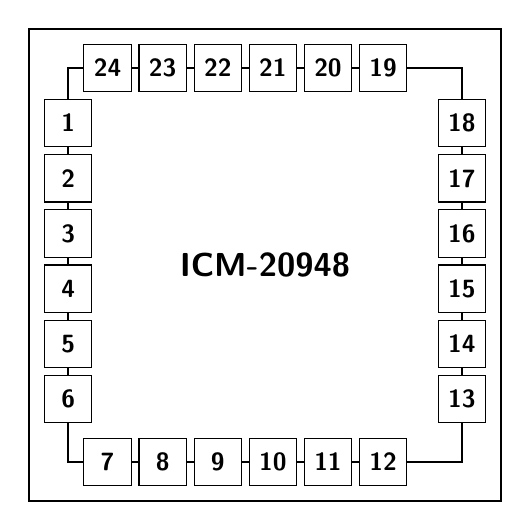
\begin{tikzpicture}[
        pin/.style={rectangle, draw, minimum height=0.6cm, minimum width=0.6cm, fill=white, font=\small\bfseries\sffamily},
        pcb/.style={draw=black, thick},
        ]
        % PCB Outline (No Fill)
        \draw[pcb] (0,0) rectangle (6,6);
        % IC Package Outline and Label
        \node[align=center, font=\large\bfseries\sffamily] at (3,3) {ICM-20948};
        \draw[thick, black] (0.5,0.5) rectangle (5.5,5.5); % Inner outline for IC package
        
        % Define pin coordinates with consistent spacing
        \foreach \x/\y/\pin in {
            1/5.5/24, 1.7/5.5/23, 2.4/5.5/22, 3.1/5.5/21, 3.8/5.5/20, 4.5/5.5/19, % Top
            0.5/4.8/1, 0.5/4.1/2, 0.5/3.4/3, 0.5/2.7/4, 0.5/2.0/5, 0.5/1.3/6, % Left
            1/0.5/7, 1.7/0.5/8, 2.4/0.5/9, 3.1/0.5/10, 3.8/0.5/11, 4.5/0.5/12, % Bottom
            5.5/1.3/13, 5.5/2.0/14, 5.5/2.7/15, 5.5/3.4/16, 5.5/4.1/17, 5.5/4.8/18 % Right
        } {
            \node[pin] (p\pin) at (\x,\y) {\pin};
        }
        
    \end{tikzpicture}
    
    \caption{ICM 20948 Schematic/Pinout Diagram (adapted from \protect\cite{TDK:2024})}
    \label{fig:ICM20948_Schematic}
\end{figure}


\clearpage







\section{Library Implementation}
\subsection{Overview of ICM20948\_WE Library}
The ICM20948\_WE library, accessible via GitHub (https://github.com/wollewald/ICM20948\_WE), provides Arduino-compatible software support for the ICM-20948 sensor. The library architecture supports both Pico and Arduino microcontroller platforms, offering a comprehensive API for sensor configuration and data acquisition.\cite{TDK:2024}

\subsection{Core Functionality}
The library implements several categories of functionality:

\subsubsection{Initialization and Configuration}
Functions are provided to configure I²C/SPI communication parameters, establish sensor measurement ranges, and enable the Digital Motion Processor (DMP). This configuration flexibility allows for application-specific optimization of sensor performance characteristics.

\subsubsection{Data Acquisition Methods}
The library exposes methods for accessing both raw and processed sensor data, including \texttt{getGyrValues()}, \texttt{getAccValues()}, and \texttt{getMagValues()}. Advanced functionality includes DMP-processed outputs such as quaternion orientation representations, which significantly simplify attitude estimation implementations \cite{Wen:2014}.

\subsubsection{Calibration Support}
Runtime calibration routines are integrated into the library, leveraging the DMP's capabilities for continuous sensor calibration. This approach aligns with recent research on adaptive filtering techniques for IMU calibration \cite{Bistrov:2012}.

\subsubsection{Interrupt Management}
The library provides support for motion detection interrupts, enabling power-efficient implementation of motion-triggered functionality—a critical requirement in battery-constrained applications.

The ICM20948\_WE library has been optimized specifically for embedded systems, with example implementations demonstrating sensor fusion techniques that are widely applied in IoT analytics research. Documentation indicates compatibility with the Arduino IDE development environment, requiring minimal adaptation for deployment on Pico microcontroller platforms.

\section{Calibration Methodology}
\subsection{Calibration Importance and Approaches}
Calibration constitutes a critical aspect of IMU implementation, addressing systematic errors including biases, scale factors, and sensor misalignment. The ICM-20948 supports multiple calibration methodologies:

\subsection{Factory Calibration}
Initial sensitivity parameters and zero-rate outputs are pre-calibrated during manufacture, significantly reducing production-line calibration requirements. This approach provides baseline accuracy for immediate deployment scenarios.

\subsection{Runtime Calibration}
The Digital Motion Processor performs continuous adjustment of gyroscope, accelerometer, and magnetometer offset parameters. This dynamic calibration process implements advanced algorithms analogous to those documented in contemporary research on adaptive filtering for inertial sensors.

\subsection{User-Initiated Calibration}
Manual calibration procedures typically involve static alignment techniques, exemplified by the 6-point tumble test methodology. These procedures are particularly effective for refining magnetometer hard-iron and soft-iron error compensation, as detailed in specialized literature on magnetic heading accuracy optimization.

\subsection{Temperature Compensation}
The ICM-20948 incorporates an on-chip temperature sensor with a sensitivity of 333.87 LSB/°C, enabling software-based temperature compensation. This capability has been validated in thermal stability studies focusing on MEMS inertial sensors.

For analytics applications, calibration data should be systematically logged and analyzed using statistical methods such as Kalman filtering to establish confidence intervals and uncertainty metrics for sensor measurements.

\section{Implementation Examples}
\subsection{Basic Data Acquisition}

{
    \captionof{code}{Basic Data Acquisition}\label{IMUICM20948:example}
    \ArduinoExternal{}{../../Code/Pico4MLPro/IMUICM20948/IMUICM20948.ino}
}

\subsection{ICM Interfacing-Arducam}

Here we have ICM Interfacing and the setup code files by Arducam sourced from their repository

\HREF{https://github.com/ArduCAM/ICM20948/tree/master}{ICM20948 Arducam} \cite{ArduCAM:ICM20948}

Here we first define the  \FILE{CMakeLists.txt}

\medskip

\lstinputlisting{../../Code/Pico4MLPro/Environment/CMakeLists.txt}

\medskip

Followed by the required header file:

\medskip

{
    \captionof{code}{Header File}\label{IMUICM20948H:example}
    \ArduinoExternal{}{../../Code/Pico4MLPro/ICM20948.h}
}

\medskip

Finally the main driver .cpp file:

{
    \captionof{code}{CPP File}\label{IMUICM20948CPP:example}
    \ArduinoExternal{}{../../Code/Pico4MLPro/ICM20948.cpp}
}

\medskip

This implementation initializes the sensor, applies automatic offset calibration, and streams data at 10Hz, providing a foundation for basic motion analytics applications.\\

\subsection{Advanced Application: Pedestrian Dead Reckoning}
A representative advanced application of the ICM-20948 is Pedestrian Dead Reckoning (PDR) for indoor navigation:

\subsubsection{System Objective}
The system aims to estimate position by implementing step detection algorithms utilizing accelerometer data, combined with heading estimation derived from fused magnetometer and gyroscope measurements.

\subsubsection{Implementation Approach}
Building upon the basic data acquisition code presented above, the implementation applies peak detection algorithms for reliable step counting. Orientation is determined by fusing gyroscope and magnetometer data through a complementary filter. The DMP can further simplify this process by providing quaternion outputs directly, reducing computational overhead on the host processor.

\subsubsection{Analytical Framework}
The system logs calibrated step length (personalized per user) and heading changes, enabling the plotting of two-dimensional trajectories. This implementation approach aligns with contemporary research on indoor navigation systems utilizing inertial measurement units \cite{Bistrov:2012}.

\section{Performance Validation}
\subsection{Accuracy Assessment Protocol}
A comprehensive validation protocol compares ICM-20948 orientation estimates against high-precision reference systems (e.g., VICON motion capture). The protocol typically encompasses 100 or more trial iterations, with success criteria defined as Root Mean Square Error (RMSE) for angular measurements below 5 degrees.

\subsection{Noise Characterization}
Noise performance evaluation requires measurement of noise spectral density under static conditions, with results validated against datasheet specifications using Fast Fourier Transform (FFT) analysis techniques. This approach provides insights into the sensor's fundamental performance limitations.

\subsection{Environmental Stability}
Temperature performance evaluation across the specified operating range (-40°C to +85°C) enables analysis of measurement drift characteristics with temperature compensation algorithms enabled. Results provide critical insights into environmental stability factors.

\subsection{Mechanical Robustness}
Shock resistance validation subjects the sensor to simulated impacts approaching the 20,000g specification limit, with subsequent verification of data integrity and calibration stability. These validation methodologies, inspired by established testing frameworks \cite{Bistrov:2012}, ensure reliability for analytics applications operating in challenging environments.

\section{Future Research Directions}
The continuing evolution of IMU sensor technology presents several promising research avenues:

\subsection{Advanced Fusion Algorithms}
Enhanced sensor fusion techniques leveraging machine learning approaches offer potential improvements in orientation accuracy under dynamic conditions . These approaches may overcome traditional limitations in environments with magnetic disturbances. \cite{Bistrov:2012}

\subsection{Power Optimization Strategies}
Further research into context-aware power management can potentially extend battery life in wearable and IoT applications. Adaptive sampling rates based on detected activity levels represent one promising approach.

\subsection{Distributed Sensing Architectures}
Networks of IMU sensors with collaborative calibration and processing capabilities present opportunities for enhanced spatial awareness in complex environments. Such architectures could enable more robust navigation in GPS-denied environments. \cite{Bistrov:2012}

\subsection{Integration with Complementary Sensing Modalities}
Fusion of IMU data with additional sensing modalities (e.g., barometric pressure, ultrasonic ranging) may address fundamental limitations of pure inertial navigation \cite{Bansal:2023}. Hybrid approaches show particular promise for extended indoor navigation applications.